\chapter{GRAPES}
Here we will talk about GRAPES \cite{GRAPES}.
Also cite the JNI guide \cite{JNIGuide}.

For the cloud support the following libraries were used: libs3
\cite{LibS3} and MySQL C Connector \cite{MySQLConnectorC}.

\section{Evaluation}

\begin{figure}[H]
  \centering
  \subfloat[][\emph{Cloud} in-degree]{
    \hspace{-70pt}
    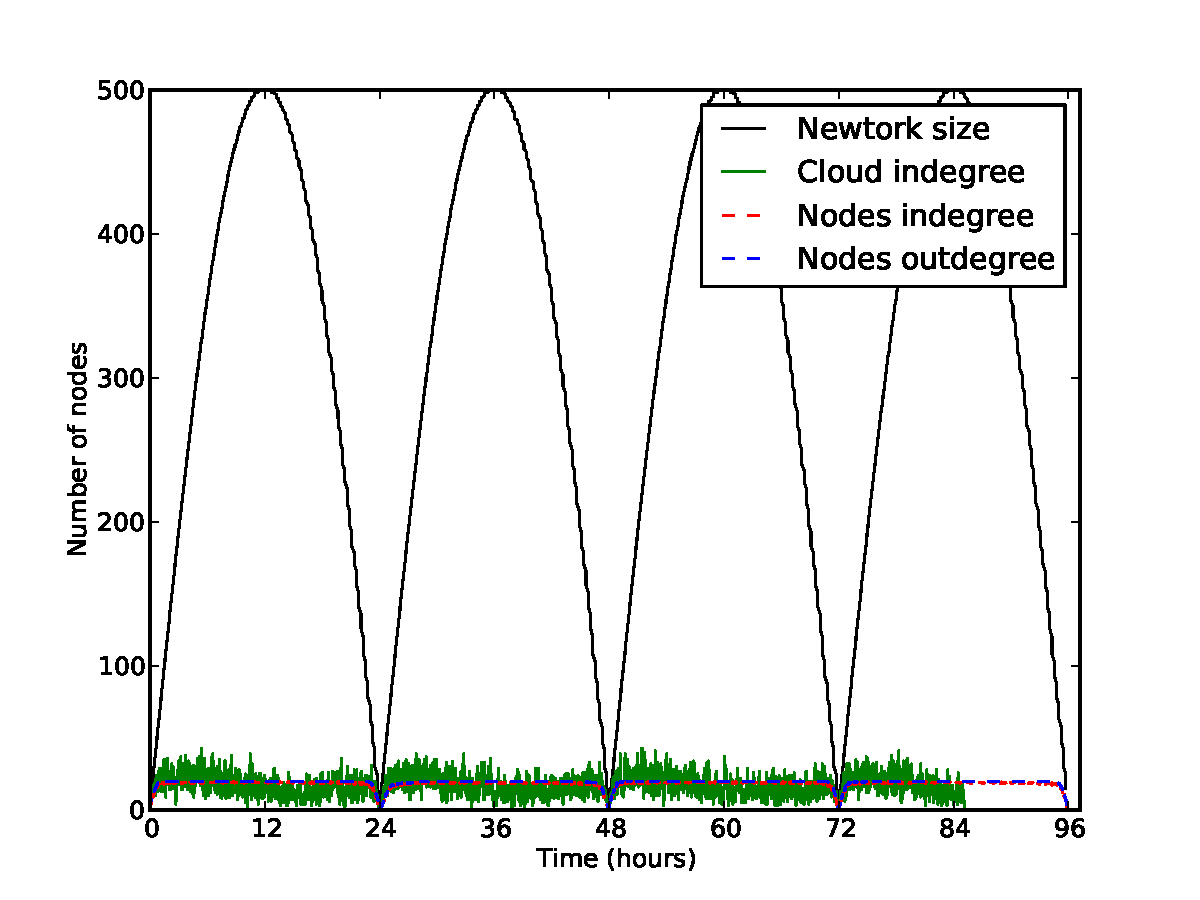
\includegraphics[width=240pt]{cloudcast-dynamic-indegree-4gg-0cloud.pdf}
    \label{fig:cloudcast-dynamic-indegree-original}
  }
  \subfloat[][\emph{Cloud} contacts]{
    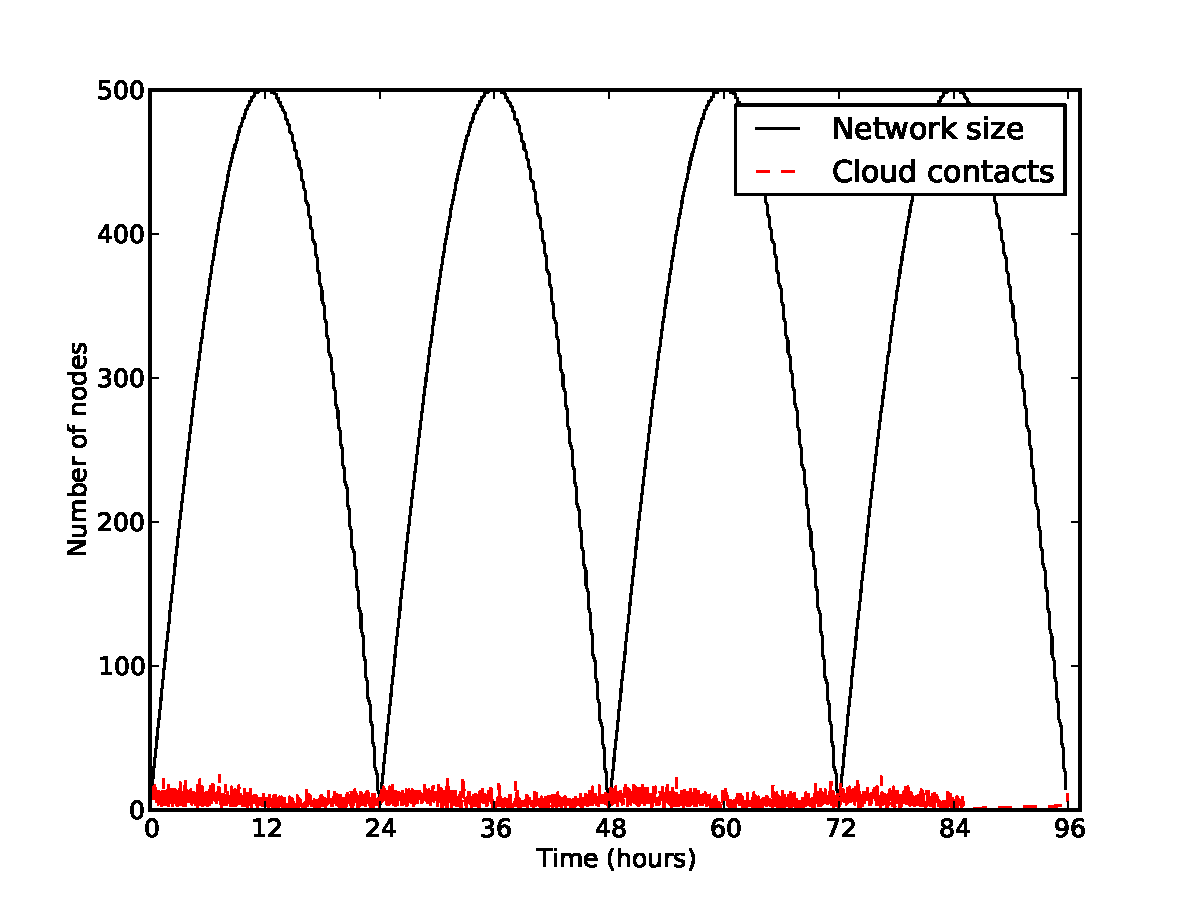
\includegraphics[width=240pt]{cloudcast-dynamic-load-4gg-0cloud.pdf}
    \label{fig:cloudcast-dynamic-load-original}
  }
  \caption{Behavior of the original \peersampling\ protocol}
  \label{fig:cloudcast-dynamic-original}
\end{figure}

\begin{figure}[H]
  \centering
  \subfloat[][\emph{Cloud} in-degree]{
    \hspace{-70pt}
    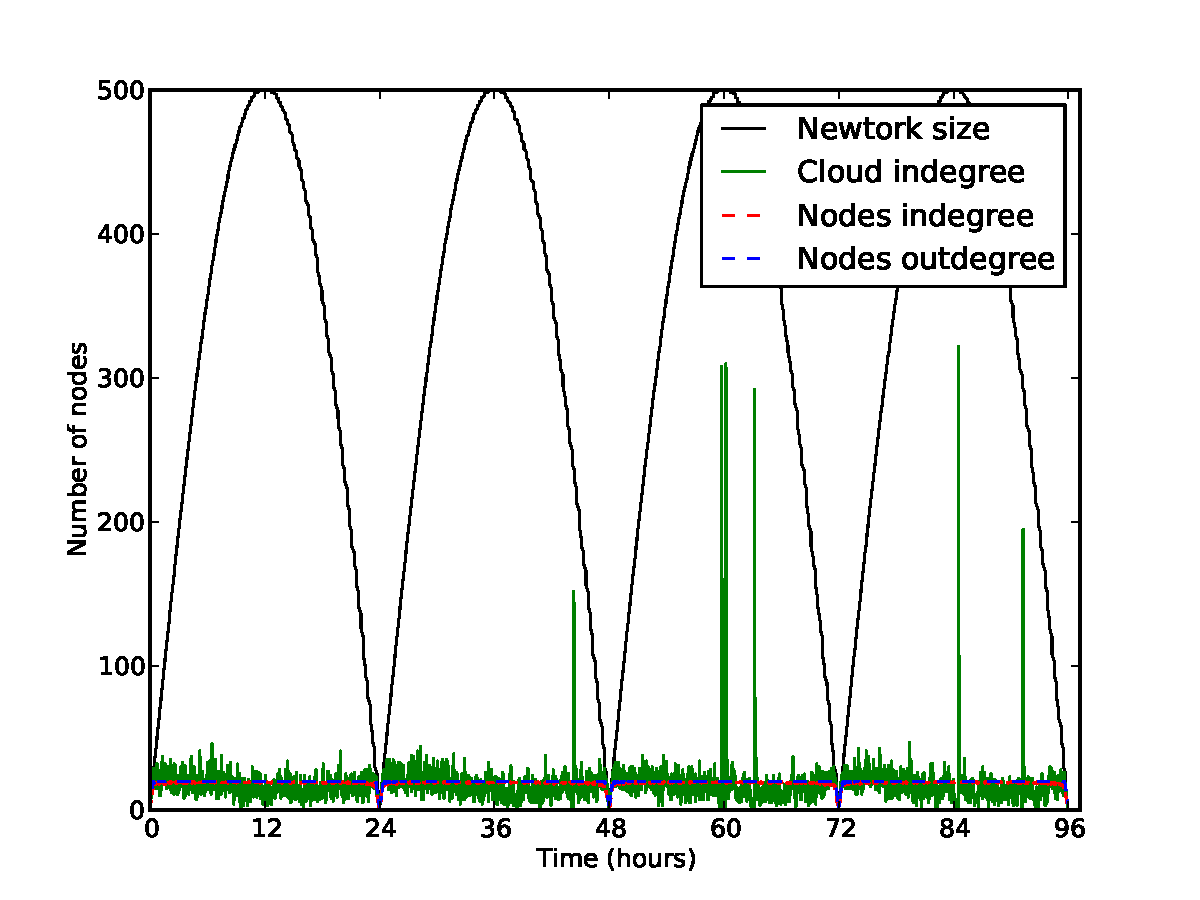
\includegraphics[width=240pt]{cloudcast-dynamic-indegree-4gg.pdf}
    \label{fig:cloudcast-dynamic-indegree-additions}
  }
  \subfloat[][\emph{Cloud} contacts]{
    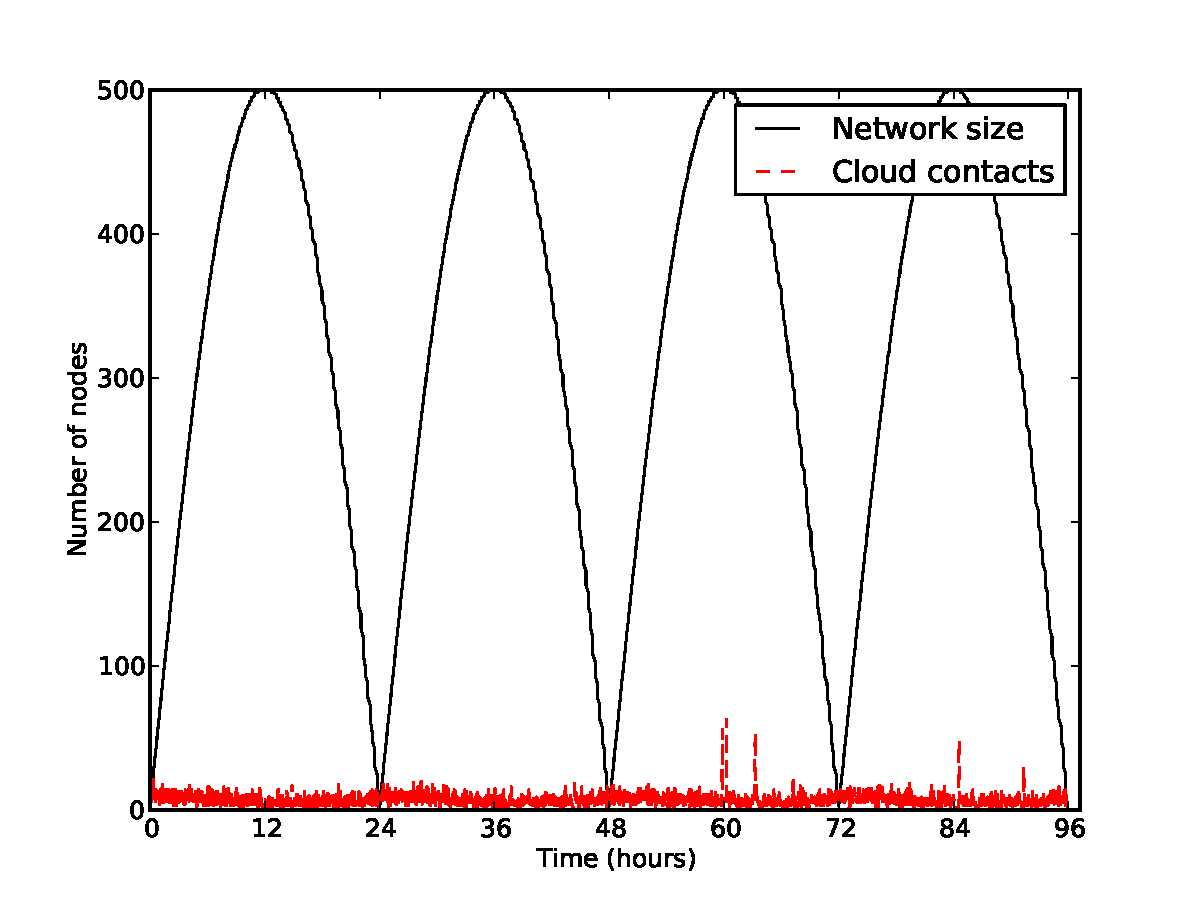
\includegraphics[width=240pt]{cloudcast-dynamic-load-4gg.pdf}
    \label{fig:cloudcast-dynamic-load-additions}
  }
  \caption{Behavior of the modified \peersampling\ protocol}
  \label{fig:cloudcast-dynamic-additions}
\end{figure}

\begin{figure}[H]
  \centering
  \subfloat[][``clean'' run]{
    \hspace{-70pt}
    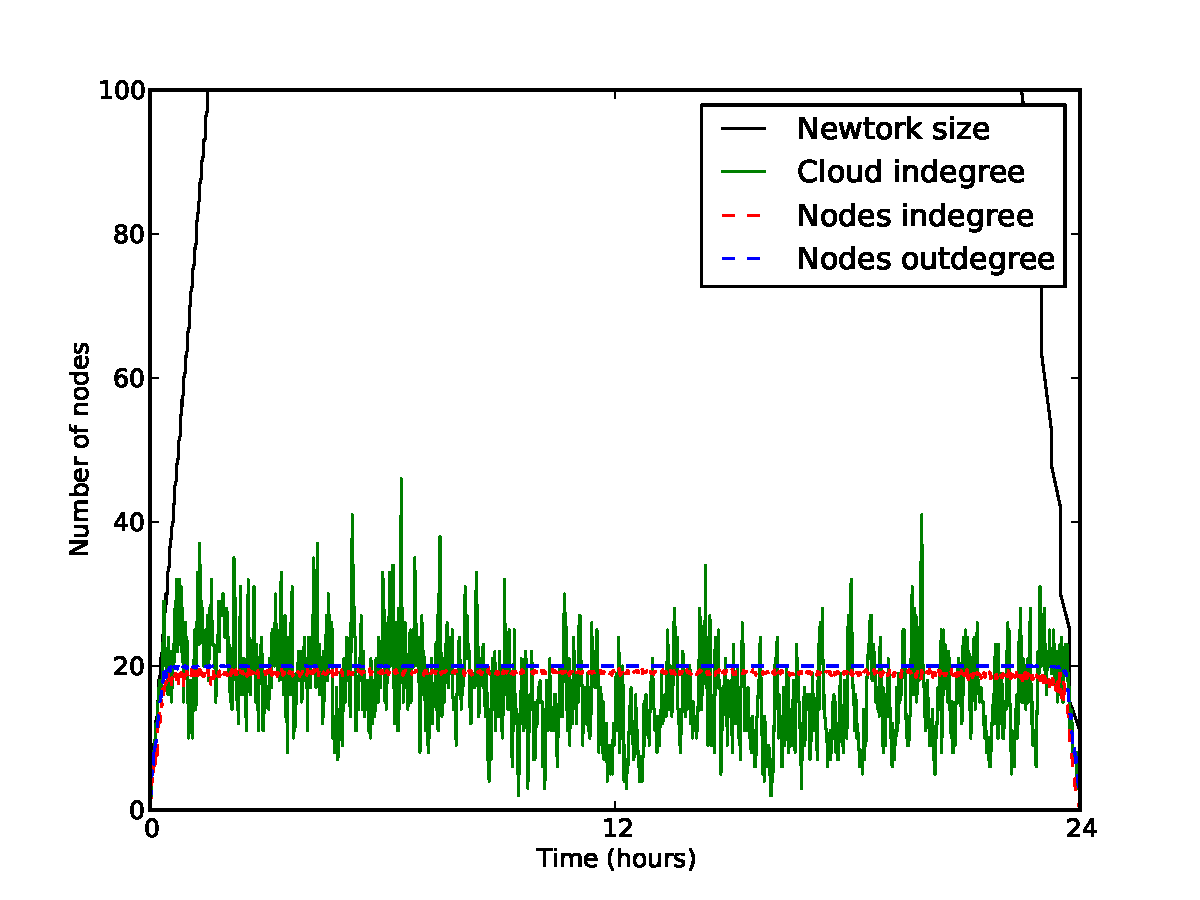
\includegraphics[width=240pt]{cloudcast-dynamic-indegree-4gg-detail-norecovery.pdf}
    \label{fig:cloudcast-dynamic-indegree-additions-detail-norecovery}
  }
  \subfloat[][Recovery mechanism in action]{
    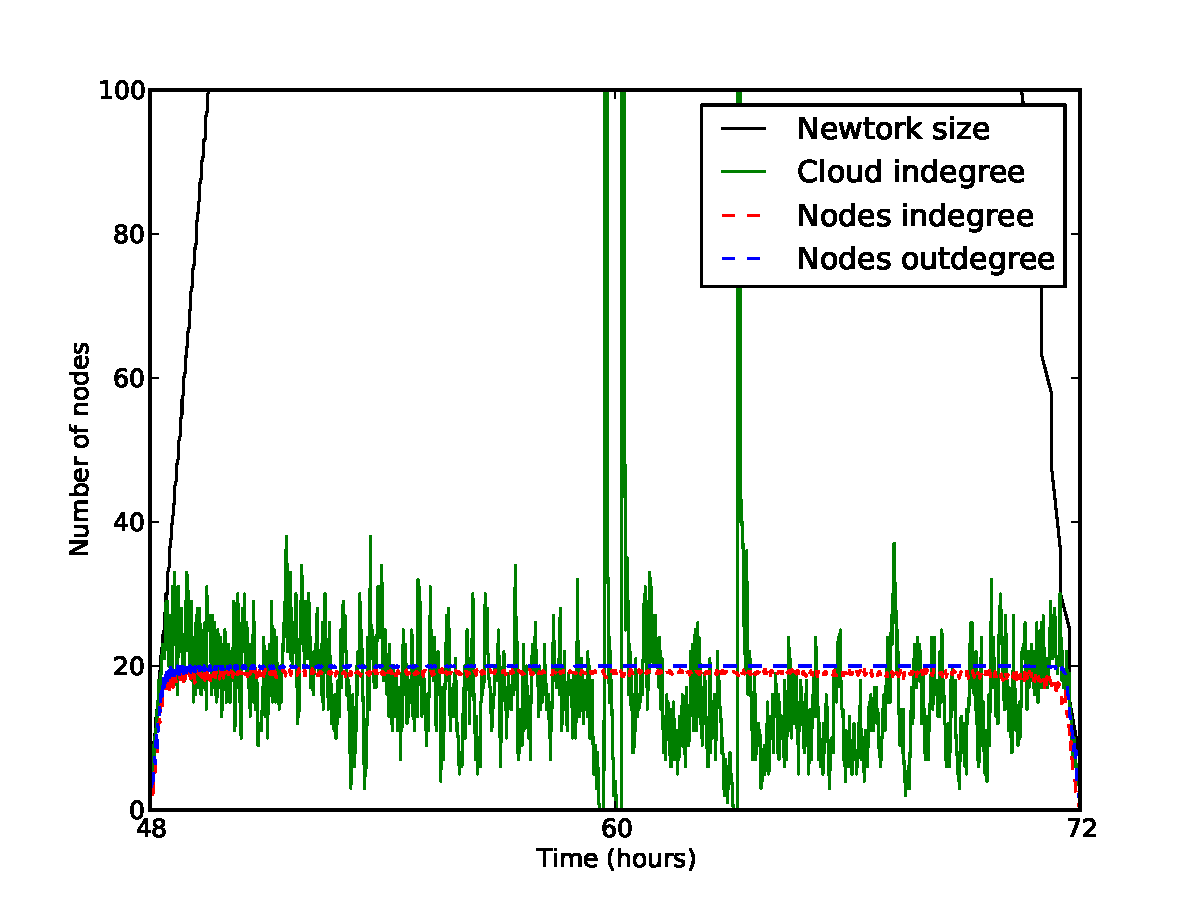
\includegraphics[width=240pt]{cloudcast-dynamic-indegree-4gg-detail-recovery.pdf}
    \label{fig:cloudcast-dynamic-indegree-additions-detail-recovery}
  }
  \caption{Zoomed in plots comparing the effects of the recovery
    mechanism on the \cloud\ in-degree}
  \label{fig:cloudcast-dynamic-indegree-additions-detail}
\end{figure}

\begin{figure}[H]
  \centering
  \subfloat[][``clean'' run]{
    \hspace{-70pt}
    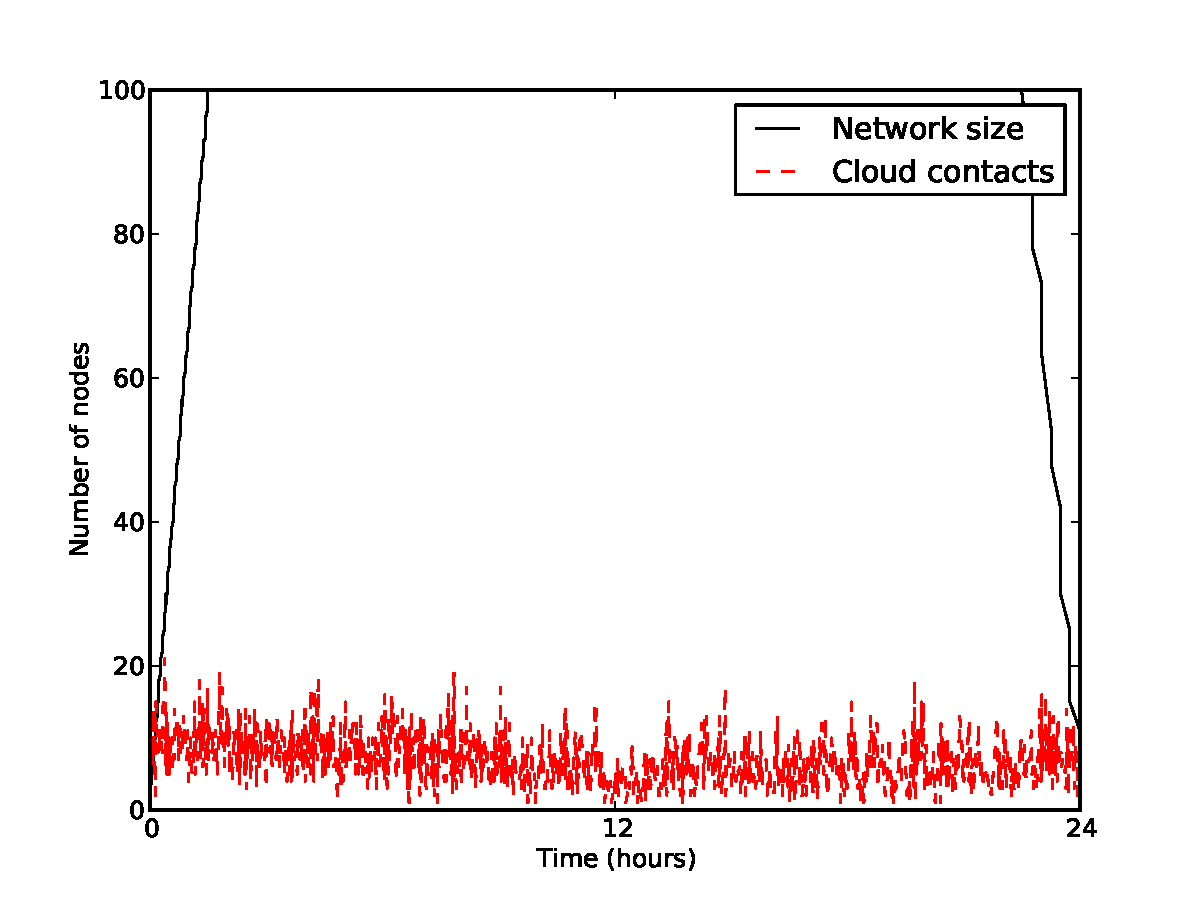
\includegraphics[width=240pt]{cloudcast-dynamic-load-4gg-detail-norecovery.pdf}
    \label{fig:cloudcast-dynamic-load-additions-detail-norecovery}
  }
  \subfloat[][Recovery mechanism in action]{
    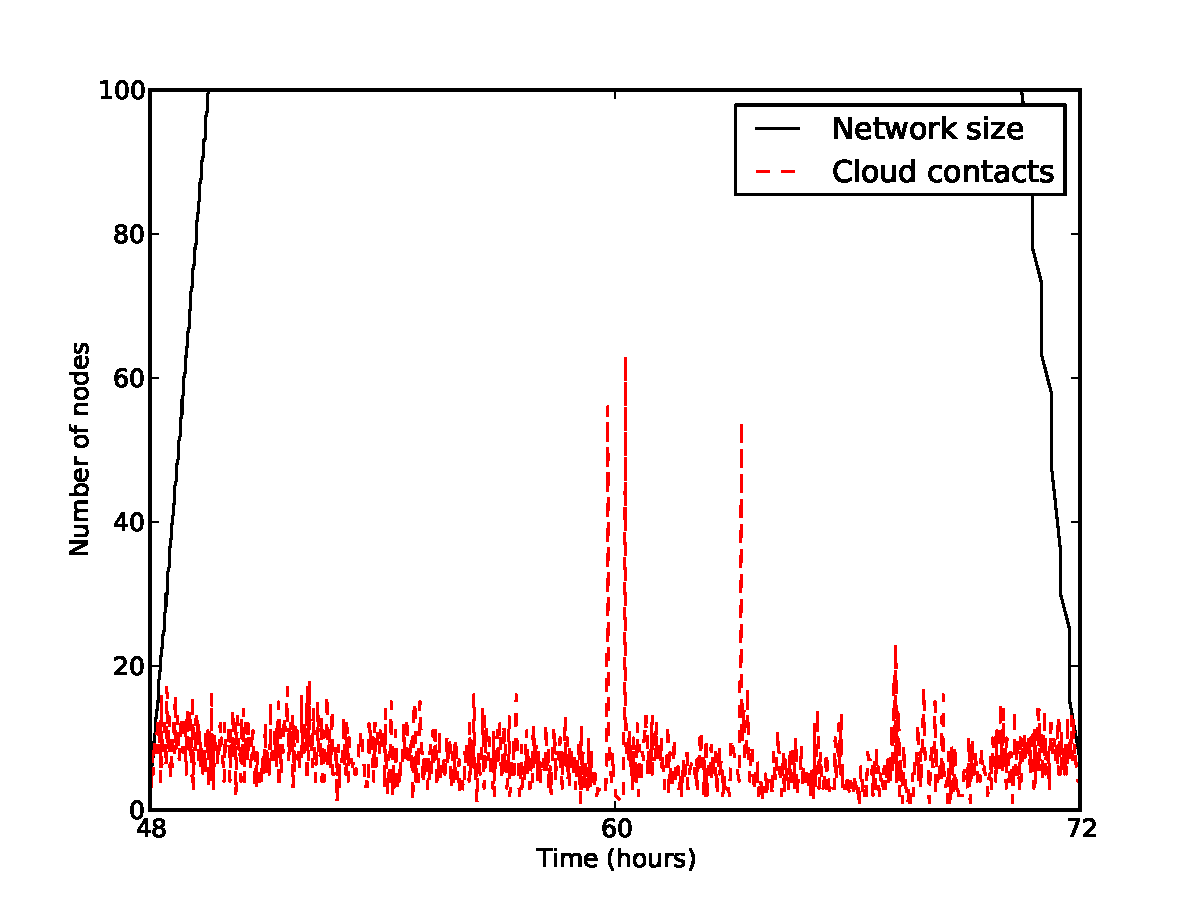
\includegraphics[width=240pt]{cloudcast-dynamic-load-4gg-detail-recovery.pdf}
    \label{fig:cloudcast-dynamic-load-additions-detail-recovery}
  }
  \caption{Detail of \cloud\ highlighting the effects of the recovery mechanism}
  \label{fig:cloudcast-dynamic-load-additions-detail}
\end{figure}

\begin{figure}[H]
  \centering
  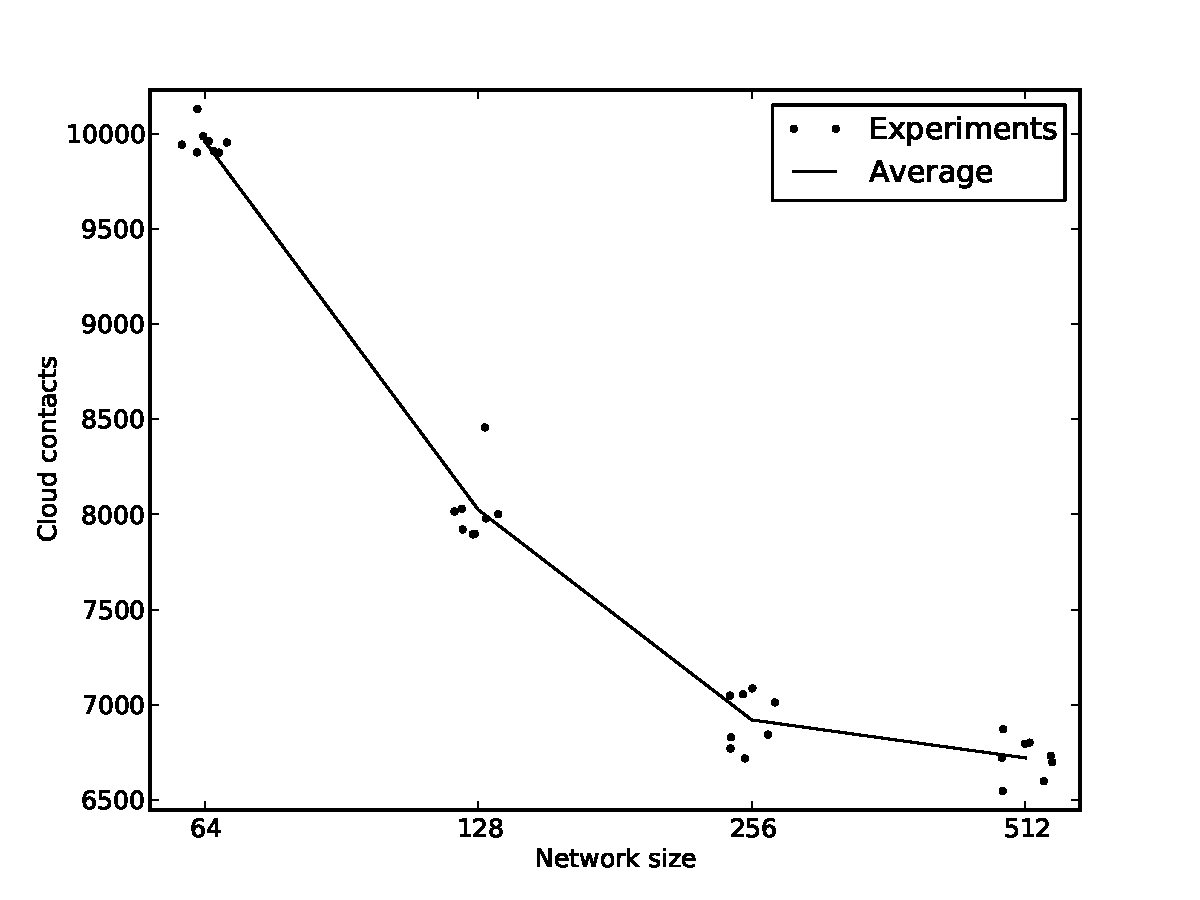
\includegraphics[width=.7\textwidth]{cloudcast-loads.pdf}
  \caption{Storage \cloud\ load for different network sizes.}
  \label{fig:cloudcast-sim-loads}
\end{figure}
